\chapter{Mixer Design}\label{ch:mixer}

	The system design chapter shows the importance of having the mixer sub-circuit first. Here we examine more in-depth how a mixer functions, different ways of realizing them, and the chosen topology in particular.

	\section{Introduction}
		\subsection{Signal multiplication}\label{sec:mixer_introduction}
			The mixer down-converts a signal by means of multiplication. The input radio frequency (RF) is multiplied with a local oscillator (LO), an external sinusoidal signal with frequency $f_{LO}$. $f_{LO}$ is selected such that one of $f_{IF}=|f_{RF}\pm f_{LO}|$ \eqref{eq:mixcos} becomes the desired down-converted signal. $f_{IF}$ is called the intermediate frequency.\autocite{maas92}

			\begin{align} \label{eq:mixcos}
				V_{RF}\cos(\omega_{RF}t)V_{LO}\cos(\omega_{LO}t)=\frac{V_{RF}V_{LO}}{2}\big[ & \cos((\omega_{RF}-\omega_{LO})t) + \nonumber \\
				& \cos((\omega_{RF}+\omega_{LO})t) \big]
			\end{align}

			The result from \autoref{eq:mixcos} requires a completely ideal multiplication device. A component with non-linear I/V-characteristics can be used for mixing, which brings about more spectral products:\autocite{bahl03}

			\begin{equation}\label{eq:poweriv}
				i = a_0 + a_1v + a_2v^2 + a_3v^3 + ... + a_Nv^N
			\end{equation}

			The current $i$ through the device depends on the sum of the two input signals $v=V_{RF}\cos(\omega_{RF}t) + V_{LO}\cos(\omega_{LO}t)$. The mixing products then become

			\begin{align}\label{eq:mixedseries}
				i = a_0 &+ a_1\left[ V_{RF}\cos(\omega_{RF}t) + V_{LO}\cos(\omega_{LO}t) \right] \nonumber \\
				& + a_2\left[ V_{RF}\cos(\omega_{RF}t) + V_{LO}\cos(\omega_{LO}t) \right]^2 + ... \nonumber \\
				& + a_N\left[ V_{RF}\cos(\omega_{RF}t) + V_{LO}\cos(\omega_{LO}t) \right]^N
			\end{align}

			The output current $i=i_{DC}+i_{IN}+i_{SPUR}$ contains a DC current term ($i_{DC} = a_0 + a_2(V_{RF}^2+V_{LO}^2)+...$), the original signals ($i_{IN}=a_1(V_{RF}\cos(\omega_{RF}t) + V_{LO}\cos(\omega_{LO}t))$) and the mixing products ($i_{SPUR}$). The second-order terms are the primary mixing products and contains the upper ($\omega_{RF}+\omega_{LO}$) and the lower ($\omega_{RF}-\omega_{LO}$) sidebands:

			\begin{align}\label{eq:mixedsecondorder}
				i_{2nd} = &a_2 \left [ \frac{1}{2}V^2_{RF}(1-\cos(2\omega_{RF}t)) + V_{RF}V_{LO}(\cos((\omega_{RF}-\omega_{LO})t) \right. \nonumber \\
				&\left. + \cos((\omega_{RF}+\omega_{LO})t)) + \frac{1}{2}V^2_{LO}(1-\cos(2\omega_{LO}t)) \right]
			\end{align}

			In this design the lower sideband is the desired intermediate frequency $\omega_{IF}$.

		\subsection{LO drive}\label{sec:mixer_lodrive}
			Regardless of topology and design choice, all mixers need an LO reference signal. This signal, or drive, is usually very large in comparison to the RF and IF signals in order to increase mixer linearity. A large LO drive will, from the RF signal's point of view, switch the mixer between on- and off-states faster, making the multiplication of the signals digital. The larger the LO drive the faster the transition between on and off states takes place. This results in more linear operation.\autocite{maas92}

			For the $P_{1dB}$ measure, not only fast on- and off-transitions are important but also the power of the LO. As explained in \autoref{sec:p1db} $P_{1dB}$ is simulated by noting at which power the gain of a component has dropped \unit[1]{dB}. When the power of the RF-signal becomes the same order of magnitude as the power of the LO drive, the LO-signal will no longer be able to switch the mixing-FET as desired. This will cause the gain to drop and thus limit $P_{1dB}$. As $IIP_3$ is closely coupled to $P_{1dB}$, this will also be limited.\autocite{kundert02}

	\section{Topologies}
		\subsection{Overview}
			The mixing functionality can be realized with a number of different mixing devices and different balanced or unbalanced designs. The literature presents two preferred devices used to multiply two signals; the diode and the transistor.\autocite{norman2002design}

		\subsection{Balanced and unbalanced mixers}
			An ordinary unbalanced mixer exhibits the behaviour where all spurious products from \autoref{eq:spurs} are present. By utilizing a balanced layout with two or more mixing elements, it is possible to suppress some of these spurious responses. There are many kinds of balanced mixers and the type determines what spurious responses are suppressed.\autocites{maas92}{dinari09}

			The downside is that additional elements must be introduced in the form of hybrids or baluns and these are often relatively large on MMICs, depending on frequency. These elements either phase shift or convert the signal between balanced and unbalanced signals.

		\subsection{Image reject mixers}
			Two mixers can be designed as an image reject mixer which cancels out the image frequency. That is the frequency which converts to the exact same IF-signal as the RF and is almost always an unwanted product. See \autoref{sec:mixer_introduction}.

			The image reject functionality is achieved, in short, when the LSB and USB (lower and upper sideband respectively) are subjected to different phase shifts in the hybrids. This makes it possible to cancel out or suppress one of the sidebands depending on the quality of the hybrids and mixers. The image reject performance is very dependant on the precision of the baluns, more specifically the degrees of phase-shift and amplitude difference.\autocite{henderson85} %Finns en artikel som visar exact vilken undertryckning man får för olika baluner

			These constructions are useful in situations when the image band lies close to the IF. In this case, the IF-signal has the frequency \unit[2.14]{GHz} and the image band starts at \unit[7.18]{GHz}. With this large distance in frequency the image is easily filtered and an image reject topology is therefore not considered.

		\subsection{Diode mixers}
			Diode mixers are realized with Schottky diodes because of their switching speed. Today diode mixers are more prevalent for high frequencies, where FETs are less potent. An advantage with diode mixers is that they do not need a bias voltage.

		\subsection{FET mixers}\label{sec:fet_mixers}
			FET mixers generally have lower noise and higher gain compared to diode mixers. There are in general two approaches to designing a FET-mixer; active or resistive mixer. MMIC processes are optimized for FET-structures, not diodes. A major advantage with FET-mixers is the inherent isolation between the LO and the IF provided by the FET.

			Active FET mixers are biased like an amplifying element and thus have a positive conversion gain while resistive mixers are biased with zero $v_{ds}$ and $v_{gs}$ below pinch-off such that the drain-source resistance is linear to the applied gate-voltage. When considering linearity, resisistive mixers are superior.\autocites{maas92,maas98}

		\subsection{Conclusion}
			Almost all MMIC mixers designed for the S band are today FET mixers. Diodes are common only when designing mixers with frequencies at least one order of magnitude higher or when using discrete components. Since high linearity is important, a FET resistive mixer is designed. To decide whether to implement it as single-ended or as singly balanced, both types are initially designed with simple ideal components. The single-balanced mixer is eventually disregarded due to its complexity and to the fact that the single-ended mixer shows adequate performance. The comparison is detailed in \autoref{sec:endvsbal}.

	\section{Design of single-ended FET resistive mixer}
		\subsection{Device}\label{sec:mixerdevice}
			As described in \autoref{sec:mixerbias}, higher LO power will result in a more linear mixer. The greater the gate width, the more LO power the FET can handle. The largest FET in the UMS process has a \unit[8$\times$75]{\mum} gate width. As it turns out, this is also the FET which gate is easiest to match to $\unit[50]{\Omega}$.\autocite{gustavsson07}

			 A shunt inductance is placed at the gate to the mixing FET in order to ensure that the FET bias point remains fixed at high LO power. The inductance is part of the matching network in the LO-amplifier.

		\subsection{Diplexer}
			The overall simplicity of the FET resistive mixer makes the diplexer the most sophisticated part and also crucial to the performance (\autoref{fig:mixerDiplexer}). Between the RF input and the mixer FET, the network has to band-pass filter the signal in order to both inhibit the IF-signal from leaking out and to suppress the radar image at $f_{image}=f_{LO}+f_{IF}$. Once the image frequency has passed this filter, it will mix down to $f_{IF}$ and from there be indistinguishable from the original signal:

			\begin{equation}
				|f_{image}\pm f_{LO}| = |f_{LO}+f_{IF}\pm f_{LO}| = \left \{
				\begin{array}{ll}
					2f_{LO}+f_{IF}, & \text{Easily filtered} \\
					f_{IF},	& \text{Harmful}
				\end{array}
				\right.
			\end{equation}

			\begin{figure}[hbt!]
				\centering
				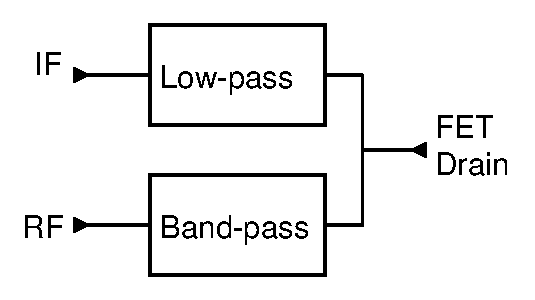
\includegraphics[width=0.5\textwidth]{fig/mixer/diplexer}
				\caption[Mixer diplexer signal path]{This diplexer consists of a low-pass filter and a band-pass filter. The signal is band-pass filtered, mixed at the FET and then low-pass filtered. Both filters are designed to match the signal to the port at the appropriate frequencies.}\label{fig:mixerDiplexer}
			\end{figure}

			Between the mixer FET and the IF output, the diplexer must low-pass filter to reject any signals above the down-mixed lower sideband frequency at $f_{IF}$. Additional filtering is done in the subsequent amplifiers.

			Besides  filtering, the diplexer has to match  both the input signal and the output signal. The input RF port is matched to \unit[50]{$\Omega$} at $\unit[2.9-3.4]{GHz}$ and the output IF port is matched to \unit[50]{$\Omega$} at \unit[2.14]{GHz}.

			The diplexer is implemented using non-resistive L-C circuits with the number of poles required to fulfil the chip specifications. The losses in the inductors add directly to the overall noise figure of the chip. The result is therefore a trade-off between filter characteristics and network simplicity.

		\subsection{Bias scheme}\label{sec:mixerbias}
			The principle of the mixer is to set the gate-source voltage $v_{gs}$ below pinch-off and then control the FET with the LO-signal. Pinch-off for the FET is $v_p\approx \unit[-0.7]{V}$. A low distortion mixer is achieved by having high LO power and thereby reducing the rise-time when the FET switches on and off. This way, less time is spent operating in regions where $v_{gs}$ is close to $v_p$ (operation at gate voltages close to $v_p$ are more non-linear). However, an LO powered too high will cause the gate to rectify and this will in turn lead to non-linear operation.\autocite{maas98} By lowering $v_{gs}$ even more below $v_p$, this can be avoided. The gate will also start to break down for too large negative gate voltages, providing a lower limit for $v_{gs}$.

			As the chip is fed a $+\unit[5]{V}$ DC, the source and drain are both raised to $|v_{gs}|$ for the mixer to experience an effective negative gate voltage and $v_{ds}=\unit[0]{V}$. The bias network is placed at the source and two large value resistors divide the voltage appropriately. No DC-current will pass through the resistors.

	\section{Schematics and layout}
		The schematic of the final resistive FET mixer is shown in \autoref{fig:mixerschematic}. The corresponding layout is found in \autoref{fig:mixerlayout}.

		\begin{figure}[hbt!]
			\centering
			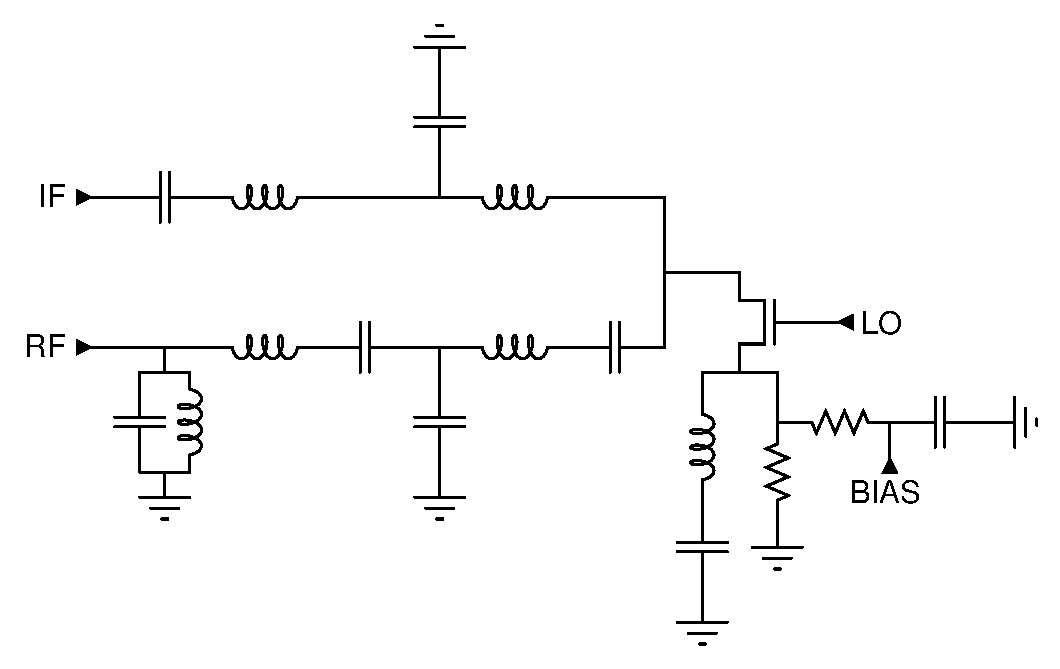
\includegraphics[width=1.0\textwidth]{fig/mixer/sch_mixer}
			\caption[Mixer schematic.]{Schematic of the mixer. Details with component values are found in \autoref{sec:detmixersch}.}\label{fig:mixerschematic}
		\end{figure}

		\begin{figure}[hbt!]
			\centering
			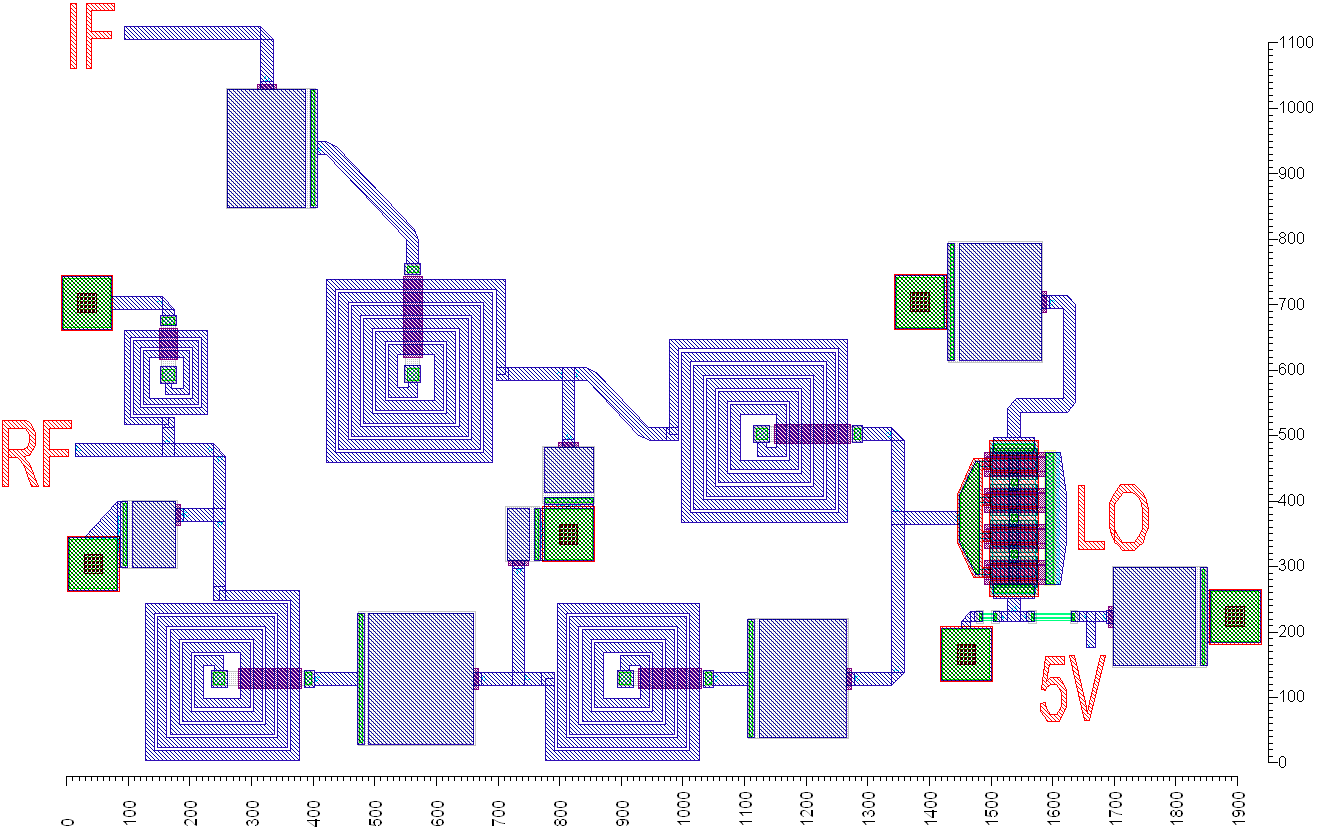
\includegraphics[width=1.0\textwidth]{fig/mixer/layout}
			\caption[Mixer layout.]{Layout of mixer.\scalemum}\label{fig:mixerlayout}
		\end{figure}

	\section{Simulation results}\label{sec:mixer}
		\subsection{Overview}
			A summary of the mixer's performance is listed in \autoref{tab:resultmixer}. Simulations are made using the LO-amplifier to provide the LO-signal. This amplifier is explained in \autoref{sec:lo_amp} but knowing it amplifies the system's LO-signal is enough to understand this mixer-chapter. All sub-circuits apart from the FETs are simulated with EM-models, see \autoref{app:emsim} for an explanation of the EM-simulations. Yield simulations are found in \autoref{sec:yield_analysis}.

			\begin{table}[hbt!]
				\caption[Simulation result of the mixer.]{Simulation results of the mixer for $LO=\unit[-2]{dBm}$ and $v_{gs}=\unit[-0.95]{V}$.\disclaimer}
				\label{tab:resultmixer}
				\centering
				\begin{tabular}{ l c c c c c c l } \toprule
					Parameter & Min. & Typ. & Max. & Min. & Typ. & Max. & Unit \\\midrule
					Frequency range RF & \multicolumn{3}{c}{2.9--3.4} & \multicolumn{3}{c}{3.1--3.3} & GHz \\
					Frequency range LO & \multicolumn{3}{c}{5.04--5.54} & \multicolumn{3}{c}{5.24--5.44} & GHz \\
					Frequency IF & \multicolumn{3}{c}{2.14} & \multicolumn{3}{c}{2.14} & GHz \\
					Return loss RF & 14 & 16 &  & 20 & 21 &  & dB \\
					Return loss Out & & 16 & & & 16 & & dB \\
					Conversion loss &  & 7.7 & 7.9 &  & 7.5 & 7.6 & dB \\
					Gain Variation & & 0.45 & 0.45 & & 0.05 & 0.05 & dB \\
					Image Rejection & 48 & 50 &  & 50 & 51 &  &  dB \\
					$P_{1dB}$ (input) & 12.7 & 13 &  & 12.7 & 13 &  & dBm \\
					$IIP_3$ (estimate) & 23 & 23 &  & 23 & 23 &  & dBm \\
					Noise figure &  & 7.7 & 7.9 &  & 7.5 & 7.6 & dB \\\bottomrule
				\end{tabular}
			\end{table}

		\subsection{Filter characteristics}
			The most important part of the diplexer filter characteristics is shown in \autoref{fig:diplexer_results}. The figure shows the EM simulated diplexer as well as a spread analysis made on the circuit model. How the spread analysis is performed is explained in-depth in \autoref{sec:yield_analysis}. For the full \unit[0--10]{GHz} frequency characteristics see Figure\autoref{fig:yielddiplexer}.

			\begin{figure}[hbt!]
				\centering
				\includerect{1.0\textwidth}{fig/yield/diplexer_zoom}
				\caption[Diplexer filter characteristics.]{Diplexer filter characteristics. The red (thick) line is the EM simulation and the blue lines correspond to the spread analysed with the circuit model. The curves marked with triangles $\triangle$ details the bandpass filter between the RF input and the mixer-FET drain. The curves marked with squares $\medsquare$ details the low-pass filter between the mixer-FET drain and the IF output.}\label{fig:diplexer_results}
			\end{figure}

		\subsection{Conversion gain and matching}
			Mixer gain (\autoref{fig:mixergain}) and input matching (\autoref{fig:mixermatch}) are calculated with the final LO-amplifier connected and using large signal analysis. The bias point does not effect neither the conversion gain nor the input matching much. The matching of the RF-port is quite independent of the LO power. The gain depends on the LO-signal which in turn depends on the LO input power. Different settings on the chip's gain block located after the first IF amplifier does not to affect the performance of the mixing part, which is why simulations with varied chip gain are not displayed. The final bias point is chosen to $v_g=\unit[-0.95]{V}$.

			\begin{figure}[hpt!]
				\centering
				\subfloat[][Conversion gain for different LO powers at $v_{gs}$=-0.95 V.]{
					\includerect{0.5\textwidth}{fig/mixer/convgainvslo}
					\label{fig:mixergainvslo}
				}
				\subfloat[][Conversion gain for different bias points $v_{gs}$ between -1.05 V and -0.75 V at $LO$=-2 dBm.]{
					\includerect{0.5\textwidth}{fig/mixer/convgainvsbias}
					\label{fig:mixergainvsbias}
				}
				\caption[Mixer conversion gain.]{Mixer conversion gain.}\label{fig:mixergain}
			\end{figure}

			\begin{figure}[hpt!]
				\centering
				\subfloat[][Input matching for different LO powers at $v_{gs}$=-0.95 V..]{
					\includerect{0.5\textwidth}{fig/mixer/matchvslo}
					\label{fig:mixermatchvslo}
				}
				\subfloat[][Input matching for different bias points $v_{gs}$ between -1.05 V and -0.75 V at $LO$=-2 dBm.]{
					\includerect{0.5\textwidth}{fig/mixer/matchvsbias}
					\label{fig:mixermatchvsbias}
				}
				\caption[Mixer RF-input matching.]{Mixer RF-input matching.}\label{fig:mixermatch}
			\end{figure}

		\subsection{Linearity}
			\autoref{fig:mixerp1dbvsbias} illustrates the compression of the conversion gain for different bias points $v_{gs}$. $P_{1dB}$ is the point where the conversion gain has dropped \unit[1]{dB} and is usually referenced to the input power compression point. $P_{1dB}$ as a function of frequency and LO input power are plotted in \autoref{fig:mixerp1db}.

			\begin{figure}[hbt!]
				\centering
				\includerect{0.7\textwidth}{fig/mixer/p1dbvsbias}
				\caption[Mixer conversion gain compression.]{Mixer conversion gain compression for different bias points $v_{gs}$. Here $LO=\unit[-2]{dBm}$ and $f=\unit[3.2]{GHz}$. The compression does not vary with the bias point.}\label{fig:mixerp1dbvsbias}
			\end{figure}

			\begin{figure}[hpt!]
				\centering
				\subfloat[][$P_{1dB}$ versus frequency for $LO$=-2 dBm and $v_{gs}$=-0.95 V.]{
					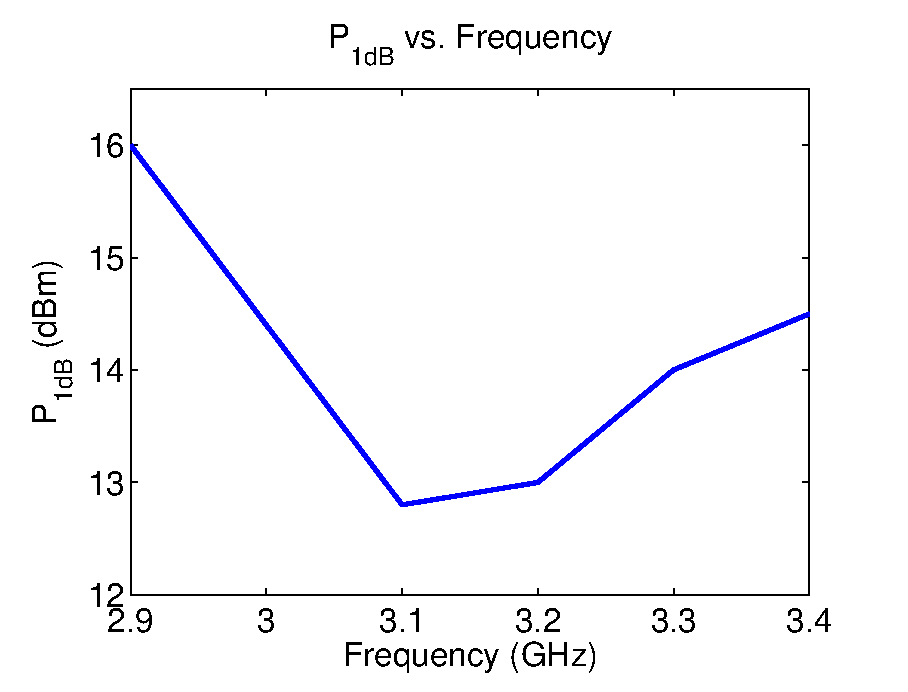
\includegraphics[width=0.5\textwidth]{fig/mixer/p1dbvsfreq}
					\label{fig:mixerp1dbvsfreq}
				}
				\subfloat[][$P_{1dB}$ versus LO power for $f$=3.2 GHz and $v_{gs}$=-0.95 V.]{
					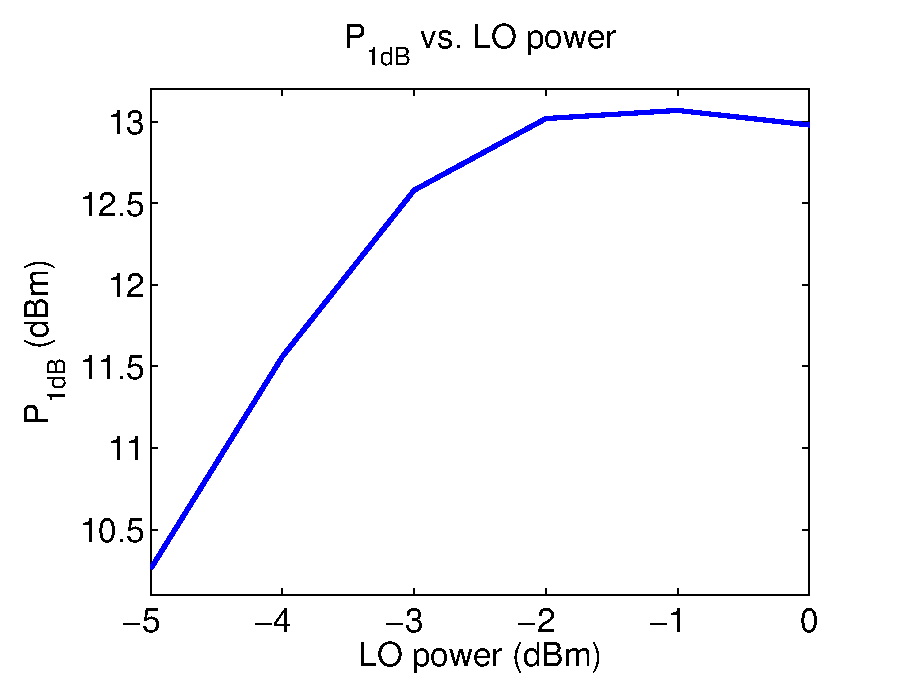
\includegraphics[width=0.5\textwidth]{fig/mixer/p1dbvslo}
					\label{fig:mixerp1dbvslo}
				}
				\caption[Mixer $P_{1dB}$.]{Mixer $P_{1dB}$ versus frequency and LO power.}\label{fig:mixerp1db}
			\end{figure}

		\subsection{Image reject}
			The conversion gain of the RF image at $f_{LO}+f_{IF}=$\unit[7.18--7.68]{GHz} is displayed in \autoref{fig:mixerimr}.

			\begin{figure}[hbt!]
				\centering
				\includerect{0.7\textwidth}{fig/mixer/imr}
				\caption[RF-image conversion gain.]{Conversion gain with the RF-image as the input signal.}\label{fig:mixerimr}
			\end{figure}

	\section{Discussion}
		As discussed in the performed topology study, there a few sophisticated designs that may give very good mixer performance. The achieved performance and the simple design of the single-ended resistive FET mixer is however undeniable. Not only does this save design effort but it also frees space on the chip, thereby saving money in yield and wafer costs. It is not surprising that the industry in general chooses this topology for high linearity mixers at these frequencies.\autocite{web:hittite}

		The noise figure in the mixer is casually considered equal to the losses. Even though this is a popular approach, there are some ways to take noise generated in the mixer into account.\autocite{kundert07} However, since the noise figure is generally somewhat lower than the losses, the conversion loss is taken as a high estimate of the noise, disregarding the more accurate noise calculations.

		Low accuracy three-tone $IIP_3$ simulations yield a result \unit[2--3]{dBm} higher than the estimates made from $P_{1dB}$. Due to their uncertainty, these results are not reported here and are only mentioned in this discussion for reference.
